%===================================================================================
% JORNADA CIENTÍFICA ESTUDIANTIL - MATCOM, UH
%===================================================================================
% Esta plantilla ha sido diseñada para ser usada en los artículos de la
% Jornada Científica Estudiantil, MatCom.
%
% Por favor, siga las instrucciones de esta plantilla y rellene en las secciones
% correspondientes.
%
% NOTA: Necesitará el archivo 'jcematcom.sty' en la misma carpeta donde esté este
%       archivo para poder utilizar esta plantila.
%===================================================================================



%===================================================================================
% PREÁMBULO
%-----------------------------------------------------------------------------------
\documentclass[a4paper,10pt,twocolumn]{article}

%===================================================================================
% Paquetes
%-----------------------------------------------------------------------------------
\usepackage{amsmath}
\usepackage{amsfonts}
\usepackage{amssymb}
\usepackage{proyecto}
\usepackage[utf8]{inputenc}
\usepackage{listings}
\usepackage[pdftex]{hyperref}
%-----------------------------------------------------------------------------------
% Configuración
%-----------------------------------------------------------------------------------
\hypersetup{colorlinks,%
	    citecolor=black,%
	    filecolor=black,%
	    linkcolor=black,%
	    urlcolor=blue}

%===================================================================================



%===================================================================================
% Presentacion
%-----------------------------------------------------------------------------------
% Título
%-----------------------------------------------------------------------------------
\title{Segundo Proyecto Estadística. Curso 2019-2020}

%-----------------------------------------------------------------------------------
% Autores
%-----------------------------------------------------------------------------------
\author{\\
	\name Daniel Alberto Garc\'ia P\'erez \email \href{mailto:d.garcia@estudiantes.matcom.uh.cu}{d.garcia@estudiantes.matcom.uh.cu}
	\\ \addr Grupo C412 \AND
	\name Leonel Alejandro Garc\'ia L\'opez \email \href{mailto:l.garcia3@estudiantes.matcom.uh.cu}{l.garcia3@estudiantes.matcom.uh.cu}
	\\ \addr Grupo C412 \AND
	\name Roberto Marti Cede\~no \email \href{mailto:r.marti@estudiantes.matcom.uh.cu}{r.marti@estudiantes.matcom.uh.cu}
	\\ \addr Grupo C412
} 

%-----------------------------------------------------------------------------------
% Tutores
%-----------------------------------------------------------------------------------
\tutors{\\Msc. Dalia Diaz Sistachs, \emph{Facultad de Matemática y Computación, Universidad de La Habana} \\}
%-----------------------------------------------------------------------------------
% Headings
%-----------------------------------------------------------------------------------
\jcematcomheading{\the\year}{1-\pageref{end}}{Daniel Alberto Garc\'ia P\'erez, Leonel Alejandro Garc\'ia L\'opez, Roberto Marti Cedeño}

%-----------------------------------------------------------------------------------
\ShortHeadings{Informe de Proyecto}{Daniel Alberto Garc\'ia P\'erez, Leonel Alejandro Garc\'ia L\'opez, Roberto Marti Cedeño}
%===================================================================================



%===================================================================================
% DOCUMENTO
%-----------------------------------------------------------------------------------
\begin{document}

%-----------------------------------------------------------------------------------
% NO BORRAR ESTA LINEA!
%-----------------------------------------------------------------------------------
\twocolumn[
%-----------------------------------------------------------------------------------

\maketitle

%===================================================================================
% Resumen y Abstract
%-----------------------------------------------------------------------------------
\selectlanguage{spanish} % Para producir el documento en Español

%-----------------------------------------------------------------------------------
% Resumen en Español
%-----------------------------------------------------------------------------------

%-----------------------------------------------------------------------------------
% English Abstract
%-----------------------------------------------------------------------------------
\vspace{0.5cm}

%-----------------------------------------------------------------------------------
% Palabras clave
%-----------------------------------------------------------------------------------

%-----------------------------------------------------------------------------------
% Temas
%-----------------------------------------------------------------------------------
\begin{topics}
	Estadística, Técnicas de Clasificación, Regresión, Anova.
\end{topics}


%-----------------------------------------------------------------------------------
% NO BORRAR ESTAS LINEAS!
%-----------------------------------------------------------------------------------
\vspace{0.8cm}
]
%-----------------------------------------------------------------------------------


%===================================================================================

%===================================================================================
% Introducción
%-----------------------------------------------------------------------------------
\section{Introducción}
%-----------------------------------------------------------------------------------
  El siguiente informe corresponde al trabajo de los autores como parte de la investigación realizada sobre los datos asignados en su segundo proyecto de la asignatura.
  
  Los datos asignados, responden a un estudio realizado sobre las respuestas correspondientes a un sensor de gases en una ciudad italiana (Data/AirQualityUCI.csv). Se tuvieron en cuenta las respuestas de los distintos terminales del sensor, así como las concentraciones de gases existentes en el ambiente.
  
  Por razones desconocidas, existen observaciones incompletas de cada una de las variables presentes en la recopilación, por lo que se hace necesario modificar las mismas para poder realizar un estudio acorde con los requerimientos de cada uno de los métodos a emplear.
  
  %Todos los recursos empleados, tanto como las imágenes presentes en este documento se encuentran adjuntos a la carpeta del proyecto.

%===================================================================================

\subsection{Descripción Inicial}
  
  Para la descripción de las características generales de los datos, se empleó el método $skim$ presente en la biblioteca $skimr$ de r, el cual brinda, entre sus valores principales, la cantidad de datos faltantes, así como los estadísticos descriptivos de cada una de las variables de la muestra. 
  
  \begin{figure}[htb]%
  	\begin{center}
  		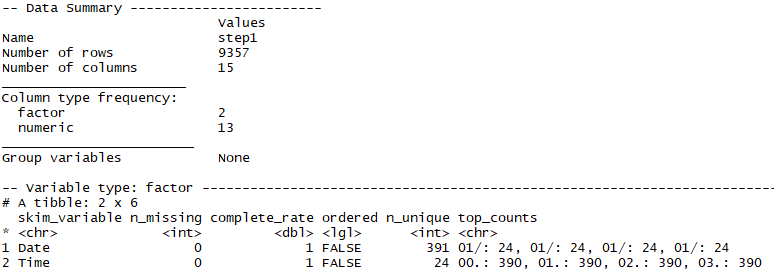
\includegraphics[width=\linewidth]{Images/skim1p1.png}
  	\end{center}
  	\caption{Descripción de la fuente de datos mediante la función skim (Parte 1).}
  	\label{fig:skim1p1}
  \end{figure}

  Como se puede apreciar de la primera mitad de los datos obtenidos de la función (Figura \ref{fig:skim1p1}), el set de datos se compone por 9357 observaciones de 15 variables. Estas se componen por 2 de tipo factor y 13 numéricas. Es importante destacar que dado que las dos variables de tipo factor, la fecha y la hora de las mediciones, se descartaron por el equipo para el análisis dado que, las mediciones se realizaron exclusivamente durante tres meses, por lo cual, no se cuenta con información suficiente para caracterizar el resto de los resultados a partir del tiempo. 
  
  \begin{figure}[htb]%
  	\begin{center}
  		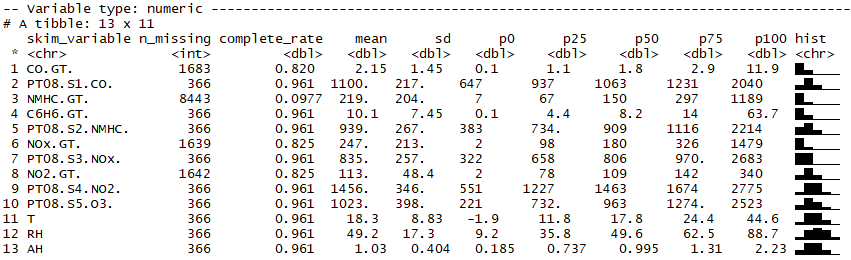
\includegraphics[width=\linewidth]{Images/skim1p2.png}
  	\end{center}
   	\caption{Descripción de la fuente de datos mediante la función skim (Parte 2).}
  	\label{fig:skim1p2}
  \end{figure}

  Centrando el análisis en la segunda parte de la respuesta obtenida de $skim$ (Figura \ref{fig:skim1p2}), resalta la cantidad de observaciones faltantes en cada una de las variables, que varían desde 366, hasta 8443. Las variables presentes, son de forma general de 3 tipos, las respuestas de los sensores a determinados compuestos del aire, la concentración de los compuestos presente, y variables generales del ambiente, temperatura, humedad relativa y absoluta.
  
  Para un mejor empleo de los datos, se completaron los datos faltantes con la media de cada una de las variables descritas en los datos.

\section{Regresión y ACP}

  El primer análisis a realizar sobre los datos fue la regresión, para ello se tuvo en cuenta la correlación existente entre cada una de las variables numéricas para corroborar si sería de utilidad realizarla.
  
   \begin{figure}[htb]%
   	\begin{center}
   		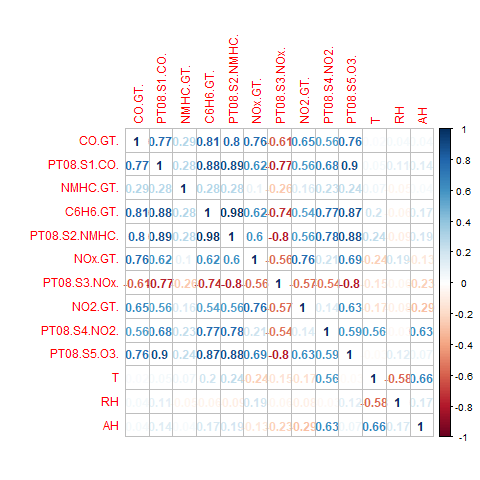
\includegraphics[width=\linewidth]{Images/correlation1.png}
   	\end{center}
   	\caption{Correlación entre las variables.}
   	\label{fig:corr1}
   \end{figure}

  La primera característica presente en los datos que se observa a partir de su correlación (Figura \ref{fig:corr1}) es que los datos de los compuestos están altamente correlacionados, por lo que la realización de una regresión lineal sobre los mismos incurriría en el problema de la multicolinealidad. 
  
  Como estrategia de solución al problema anterior, se decidió agrupar los datos por sus componentes principales, para así, reducir los datos de ser posible y poder dar una interpretación mas clara a la regresión. Como no se dispone de interés especial por alguna variable se decidió empelar la variable de la respuesta del sensor número 4 relacionado con el dióxido de nitrógeno ($PT08.S4.NO_2$) debido a que presenta pocos datos faltantes y es las mas correlacionada con los datos disponibles.
  
 \subsection{ACP} 
 
  A continuación (Figura \ref{fig:acp1}) se encuentran todas las posibles componentes resultantes del desgloce (Buscar como se escribe) de los datos.
 
 \begin{figure}[htb]%
 	\begin{center}
 		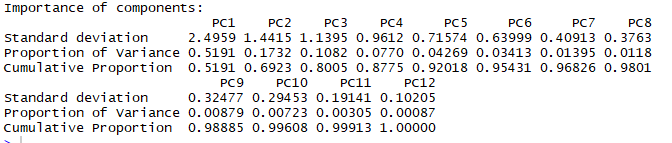
\includegraphics[width=\linewidth]{Images/acp1.png}
 	\end{center}
 	\caption{Posibles componentes principales.}
 	\label{fig:acp1}
 \end{figure}

  Se tuvieron en cuenta dos criterios tomados de la literatura para la selección de las componentes principales, un criterio de $porcentaje$ que debería superar como mínimo el 70\% de los datos y el criterio de $Kaiser$. Como podemos observar en las componentes (Figura \ref{fig:acp1}) con las dos primeras ya se cumple el criterio de mas del 70\% de los datos, pero para cumplir también con $Kaiser$ se extendieron las componentes hasta la tercera.
  
  \subsubsection{Descripción de las componentes} \label{acp:description}
  
  Para poder describir detalladamente las características de cada una de las tres componentes en las que se aglomeran los datos de estudio se analizó su matriz de valores propios. (Figura \ref{fig:acp2})
  
  \begin{figure}[htb]%
  	\begin{center}
  		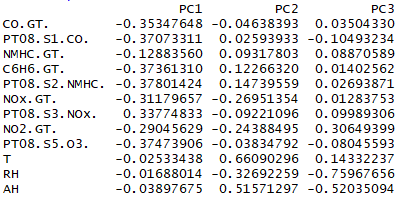
\includegraphics[width=\linewidth]{Images/acp2.png}
  	\end{center}
  	\caption{Valores propios de las componentes principales.}
  	\label{fig:acp2}
  \end{figure}

  La primera componente se caracteriza por bajos valores de la concentración de todos los compuestos presentes en el estudio con excepción los hidrocarburos no metánicos ($NMHC.GT$), así como bajos valores de respuesta de todos los sensores, exceptuando a la variable dependiente. Esta componente, la mas numerosa de las analizadas describe el comportamiento mas común de los datos, este resultado puede estar determinado por que las muestras se obtuvieron en una sola zona de la ciudad, en una sola ciudad o en un intervalo de tiempo donde no varían mucho.
  
  La segunda componente se caracteriza por valores altos de la temperatura y humedad relativa. Esta componente describe las situaciones de las horas cercanas al mediodía donde la temperatura es mas elevada.
  
  La última componente se caracteriza por altos valores de la humedad relativa y absoluta. Dada la presencia de altos valores de humedad tanto en la 2da como en la 3ra componente se puede llegar a la conclusión que algunas de las mediciones se encontraron en temporada de lluvias u ocurrió algún evento climatológico.
  
  \subsection{Regresión} 
  
  Posterior a la definición de las componentes se dispuso la creación de un modelo de regresión múltiple, donde la variable dependiente se tomó como la respuesta del cuarto sensor a la concentración de $NO_2$, y como variables independientes las 3 componentes resultantes del $ACP$. Se comprobó una vez mas la utilidad de realizar la regresión mediante los gráficos de dispersión y correlación (Figuras \ref{fig:pairs1} y \ref{fig:correlation2}).
  
  \begin{figure}[htb]%
  	\begin{center}
  		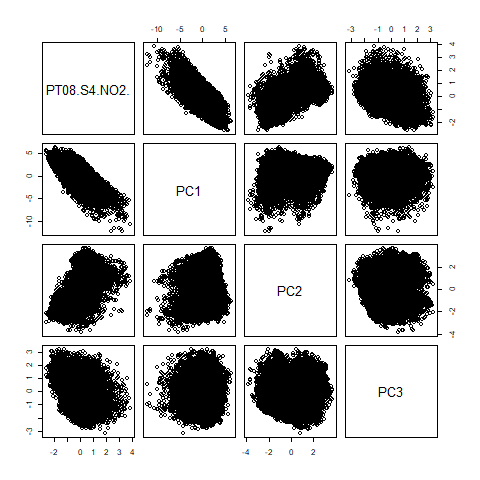
\includegraphics[width=\linewidth]{Images/pairs1.png}
  	\end{center}
  	\caption{Gráfico de dispersión.}
  	\label{fig:pairs1}
  \end{figure}

  Del gráfico de dispersión (Figura \ref{fig:pairs1}), podemos percatarnos de la correlación inversa de la variable dependiente con la primera componente, así como su relacion débil pero lineal con la segunda. Ambos datos se esclarecen con la gráfica de correlación (Figura \ref{fig:correlation2}).

  \begin{figure}[htb]%
  	\begin{center}
  		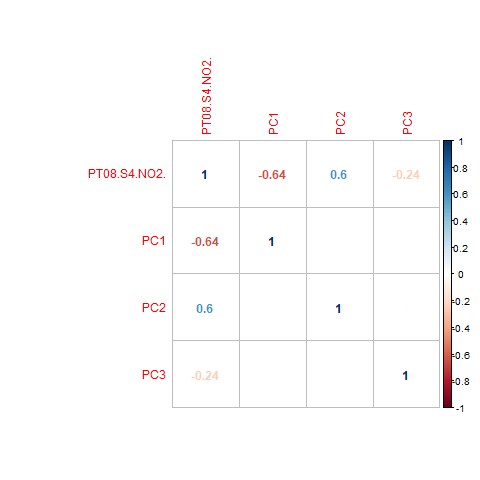
\includegraphics[width=\linewidth]{Images/correlation2.png}
  	\end{center}
  	\caption{Gráfico de correlación.}
  	\label{fig:correlation2}
  \end{figure}

  Otro detalle significativo se deduce de los resultados de la clasificación en componentes principales, dado que brindan una segmentación en variables independientes, como se muestra en la figura \ref{fig:correlation2}. Finalmente antes de la realización de la regresión se tomó como consenso la admisión de los valores de las correlaciones de la primera y segunda componentes con la variable dependiente como lineales.
  
  \begin{figure}[htb]%
  	\begin{center}
  		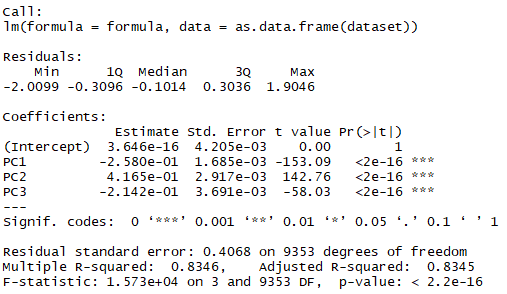
\includegraphics[width=\linewidth]{Images/regression1.png}
  	\end{center}
  	\caption{Resumen de la regresión.}
  	\label{fig:regression1}
  \end{figure}

  Los resultados obtenidos del modelo se reflejan en la figura \ref{fig:regression1}. De los mismos se deduce la siguiente ecuación para determinar el valor de la respuesta del sensor a la concentración de dióxido de nitrógeno.
  
  \begin{center}
  	$PT08.S4.NO_2$ = $-0.26$ * $PC1$ + $0.42$ * $PC2$ - $0.22$ * $PC3$
  \end{center}

  Uno de los factores a tener en cuenta es la estandarización de los datos durante el proceso de clasificación, por lo que su efecto se ve reflejado en la ausencia del término independiente en la ecuación de regresión.
  
  En el modelo propuesto por cada unidad de decremento de todas las variables presentes en la componente 1 (Ver sección \ref{acp:description}), el valor de respuesta del sensor al dióxido de nitrógeno disminuye en 0.26 unidades aproximadamente. Por cada unidad de incremento en la temperatura y la humedad absoluta, se incrementa la respuesta del sensor en aproximadamente 0.42 y finalmente por cada unidad de incremento de la humedad relativa y absoluta se decrementa la respuesta en 0.22 unidades aproximadamente. 
  
  La precisión del modelo medida en términos del valor de $R-ajustado$ es de 0.8343 lo cual es bastante alto tomando en consideración los datos faltantes y el desprecio de datos resultante del $ACP$. El $p-valor$ de la prueba de $F-statistic$ es menor que 0.05 por lo que podemos asegurar que nuestro modelo produce resultados. El error residual es de 0.4. Todas las variables independientes son de importancia para la estimación de la variable dependiente.
  
  \subsubsection{Análisis de los supuestos de la regresión}
  
  \begin{enumerate}
  	\item Las variables independientes no están correlacionadas.
  	\item La media y la suma de los errores es cero.
  	\item Los errores tienen distribución normal.
  	\item Los errores son independientes.
  	\item La varianza de los errores es constante.
  \end{enumerate}

  El primer requisito de los supuestos del modelo se cumple al emplear como variables independientes el resultado de aplicar el $ACP$. (Ver gráfico \ref{fig:correlation2}).
  
  Se obtuvo del modelo que la suma de los errores es $4.3e-13$ y la media de los mismos es $4.6e-17$ por lo que podemos asegurar que la media y la suma de los errores es 0.
  
  \begin{figure}[htb]%
  	\begin{center}
  		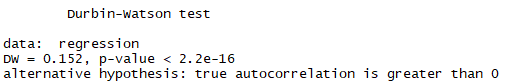
\includegraphics[width=\linewidth]{Images/dwtest.png}
  	\end{center}
  	\caption{Prueba de Durwin-Watson.}
  	\label{fig:dwtest}
  \end{figure}
  
  Como se puede observar del resultado de la prueba de independencia de Durwin-Watson (Figura \ref{fig:dwtest}), el $p-valor << 0.05$ por lo que podemos rechazar la hipótesis nula y los errores son dependientes. Esto incumple con los supuestos delo modelo por lo que se termina su análisis y se descarta su empleo.
  
  En la carpeta de imágenes adjunta al proyecto se pueden visualizar los resultados obtenidos de la normalidad de los errores y la homocedasticidad.
  
\section{Cúlster, Kmeans y Árbol de Desición}
  
  Para el análisis de tipo clúster se tomaron en cuenta los resultados obtenidos del $ACP$, por lo que el número de particiones del clúster jerárquico se fijo a 3, pero también. se valoró la inclusión de 2 clústers como se puede apreciar en el dendograma (Figura \ref{fig:cluster1})
  
  \begin{figure}[htb]%
  	\begin{center}
  		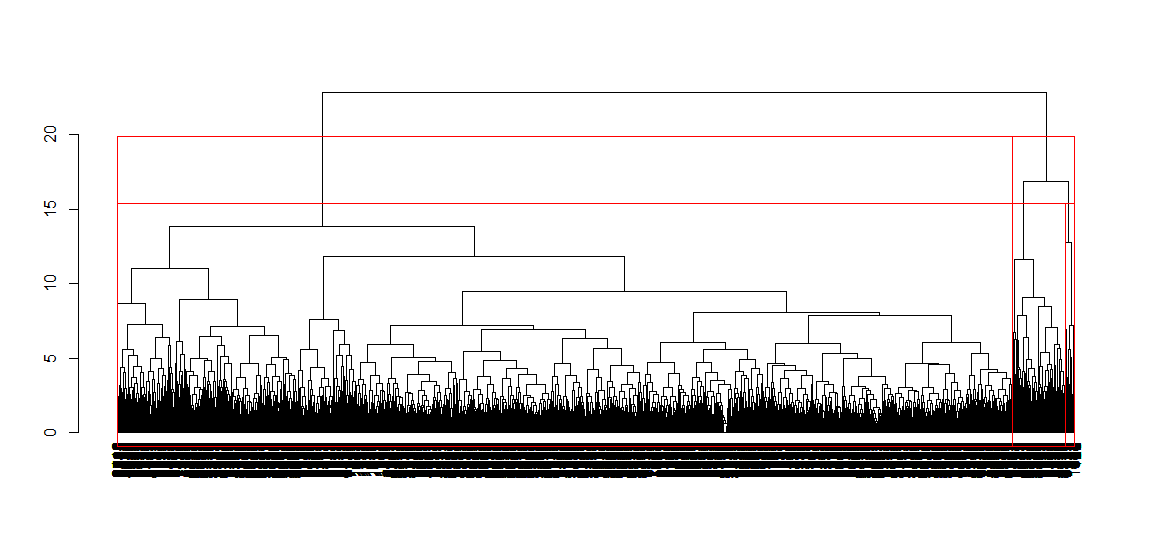
\includegraphics[width=\linewidth]{Images/cluster2.png}
  	\end{center}
  	\caption{Dendograma del clúster jerárquico con 2 y 3 particiones de los datos.}
  	\label{fig:cluster1}
  \end{figure}
  
  Uno de los detalles que más denotan de la gráfica anterior recae en la gran acumulación de datos en la primera partición, posiblemente se deba a que los datos son tomados de una misma zona y no variaron mucho durante los tres meses del estudio.
  
  Tomando los resultados anteriores, se dispuso de la ejecución del algoritmo $Kmeans$ cuyo resultado se puede observar en la figura \ref{fig:kmeans1}. Primero se intentó una aproximación de dos particiones, pero se obtuvo una similitud entre componentes de un 33\%, por lo que se decidió emplear tres particiones para el resultado final del algoritmo.
  
  \begin{figure}[htb]%
  	\begin{center}
  		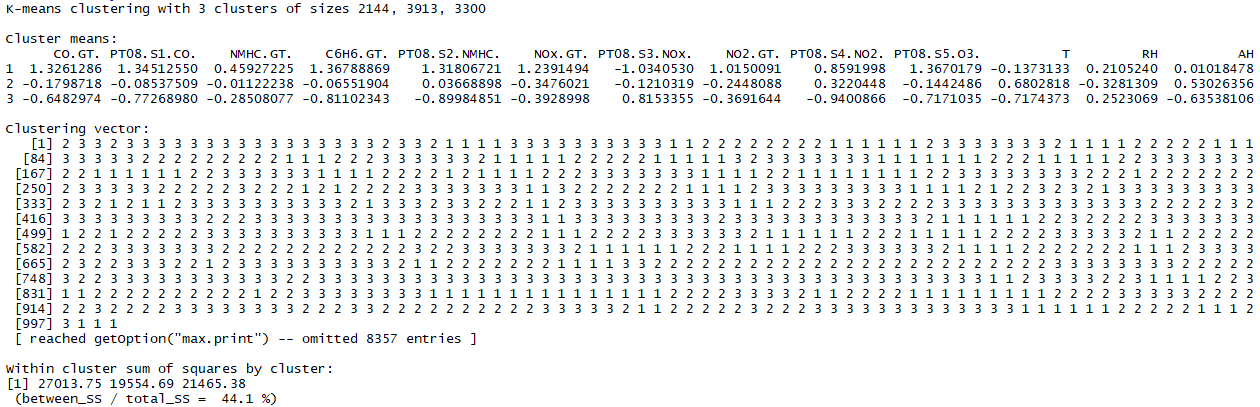
\includegraphics[width=\linewidth]{Images/kmeansummary1.png}
  	\end{center}
  	\caption{Resumen de la aplicación de Kmeans.}
  	\label{fig:kmeans1}
  \end{figure}
  
  Para concluir con el proceso de $Kmeans$, se analizó también de forma gráfica la distribución de los datos obtenidos (\ref{fig:kmeans2}). La distribución de los datos en tres particiones de tamaños 2144, 3913 y 3300, se ve reflejado en la gráfica. El color rojo se asigna a la 2da componente, el negro a la tercera y el verde a la primera.
  
  \begin{figure}[htb]%
  	\begin{center}
  		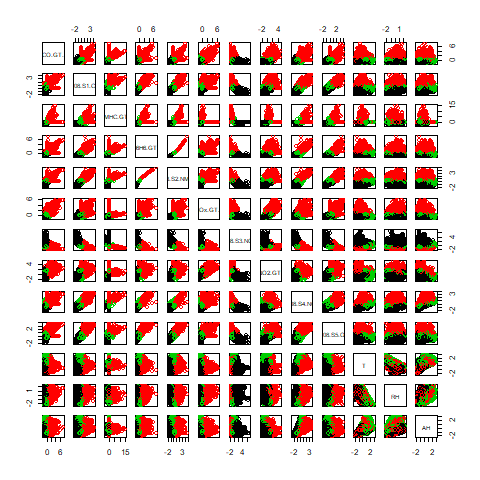
\includegraphics[width=\linewidth]{Images/kmeans1.png}
  	\end{center}
  	\caption{Forma gráfica de Kmeans por variable.}
  	\label{fig:kmeans2}
  \end{figure}

  Tras el intento fallido mediante la regresión de establecer una relación entre la respuesta del sensor al dióxido de carbono, se centró el estudio del árbol de decisión sobre el mismo (Figura \ref{fig:pt08}). Pero tras
  analizar el error de clasificación, este resultó casi uno, de un 99.98\%, por lo que se desechó el mismo. Posteriormente, se analizó otro árbol de clasificación, esta vez con una variable con la mayor muestra de datos, el Tiempo. El experimento resultó una vez más con error similar al caso anterior por lo que también se desechó esta aproximación.
  
  \begin{figure}[htb]%
  	\begin{center}
  		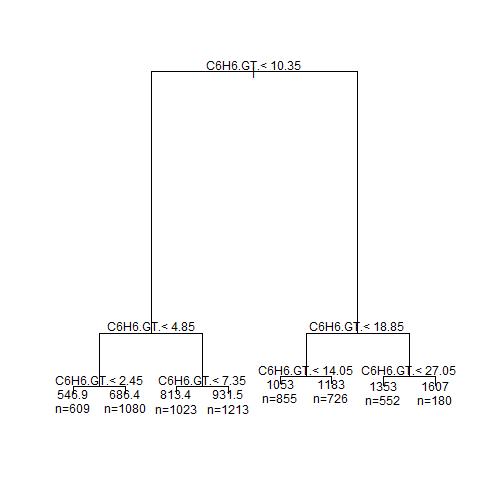
\includegraphics[width=\linewidth]{Images/decision_tree_second_try.png}
  	\end{center}
  	\caption{Árbol de decisión sobre la variable PT08.S2.NMHC.}
  	\label{fig:pt08}
  \end{figure}

\newpage

\section{ANOVA}
 Se intentó finalmente realizar el test ANOVA sobre los datos para estudiar el factor sensor dado que todos los sensores miden algún tipo de óxido.
 
 Primeramente se analizó la gráfica de medias y diagrama de cajas simultáneo como se muestra a continuación. 
 
   \begin{figure}[htb]%
  	\begin{center}
  		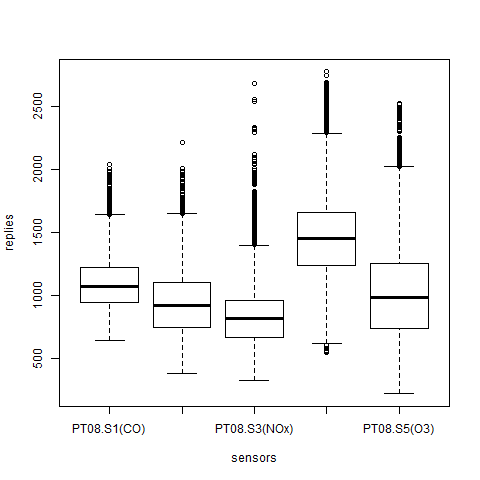
\includegraphics[width=\linewidth]{Images/boxplot_anova.png}
  	\end{center}
  	%\caption{Diagrama de cajas simultáneo.}
  	\label{fig:Cajas}
  \end{figure}

 Las etiquetas corresponden a cada uno de los sensores; y el eje replies las concentraciones del compuesto correspondiente.

 Se aprecia diferencia entre cada una de las medias de los sensores, así como la presencia de datos aislados cuya cantidad es notable. Este fenómeno de la gran cuantía de datos aislados podemos afirmar que se debe a la sustitución de cada dato faltante por la media del resto. Estos datos remplazados se agrupan cerca de la media (porque tiene el mismo valor) y resulta que los datos reales quedan aislados. Se asegura entonces que el resultado del test va a arrojar diferencias entre las medias.
 
 \subsection{Hipótesis y Modelo Estadístico}
 
 El modelo estadístico escogido fue le de Clasificación Simple. Tenemos claramente el factor
 sensor, el cual fue previamente seleccionado para saber si existe diferencia entre la concentración
 media de los compuestos.
 
 ¿ Existe diferencia entre la concentración promedio medida por los sensores ?
 
 La respuesta a esta pregunta es el resultado de contrastar las hipótesis:
 $$H_0: \mu_1 = \mu_2 = \mu_3 = \mu_4 = \mu_5 $$
 $$H_1: \mbox{existen}\; 1 \le i < j \le 5 \;\mbox{tales que}\; \mu_i \ne \mu_j $$
 Donde $\mu_i$ denota la concentración media medida por el sensor $i$. Como estudiamos en conferencias si denotamos $y_{ij}$ como la concentración medida por el sensor $i$ en la r\'eplica $j$, la misma se puede escribir como: $y_{ij} = \mu_i + e_{ij}$, siendo $e_{ij}$ el error experimental o la perturbaci\'on.
 
 \subsection{Diferencias entre la concentración promedio medida	por cada sensor}
 
 Realizamos la prueba de hip\'otesis planteada anteriormente para un nivel de significaci\'on no especificado. 
 Nuevamente apoy\'andonos en el lenguaje r. Los resultados de la misma son los siguientes (figura \ref{fig:anova}).
 
 \begin{figure}[h!]
 	\centering
 	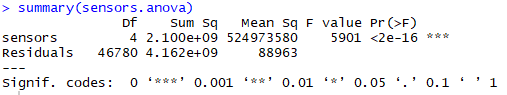
\includegraphics[width=\linewidth]{Images/anova_summary.png}
 	\caption{Prueba de Hip\'otesis}
 	\label{fig:anova}
 \end{figure}
 
 Los resultados arrojan un $p$-\textit{value} menor a $2 \times 10^{-16}$, el cual es prácticamente $0$, pues el valor
 es cercano al meno n\'umero representable en la aritm\'etica flotante de r. Con lo cual cualquier nivel
 significaci\'on $\alpha \in \{0.01, 0.1, 0.5\}$ es v\'alido, con lo cual rechazamos la hip\'otesis nula y podemos afirmar que existe diferencia entre la concentración promedio medida por cada sensor.
 
 La mayor concentraci\'on la tiene el 4to sensor. Dado el \'exito de la prueba de hip\'otesis, partimos de
 la existencia de una diferencia, ahora bien, la evidencia visual nos muestra que la media del sensor 4 es superior, incluso si tenemos en cuenta los extremos del intervalo, estos tambi\'en son
 superiores a los de los otros sensores.
 
 \subsection{Supuestos de normalidad y de igual varianza}
 
 La validez de los resultados obtenidos en cualquier an\'alisis de varianza queda supeditada a que los
 supuestos del modelo se cumplan. Estos supuestos son:
 
 \begin{enumerate}
 	\item Los $e_{ij}$ siguen una distribuci\'on normal con media cero.
 	\item Los $e_{ij}$ son independientes entre s\'i.
 	\item Los residuos de cada tratamiento tienen la misma varianza $\sigma^2$.
 \end{enumerate}

 \subsubsection{Pruebas Gráficas}
 
  Comenzando por las pruebas gr\'aficas. Los resultados se muestran a continuaci\'on en las figuras \ref{fig:anova_residuals}, \ref{fig:anova_qq} y \ref{fig:anova_hist}.
 
 \begin{figure}[h!]
 	\centering
 	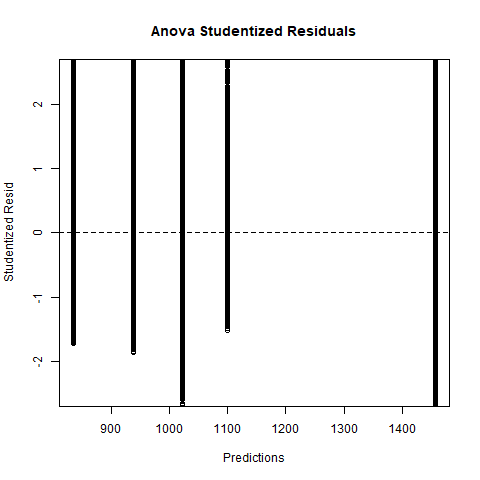
\includegraphics[width=\linewidth]{Images/anova_studentized_residuals.png}
 	\caption{Residuos}
 	\label{fig:anova_residuals}
 \end{figure}
 
 Primeramente, en el gr\'afico estandarizado de residuos (figura \ref{fig:anova_residuals}), notamos los puntos
 muy dispersos, sin patrón aparente, por lo que podríamos aseguramos el supuesto de varianza constante.
 
 \begin{figure}[h!]
 	\centering
 	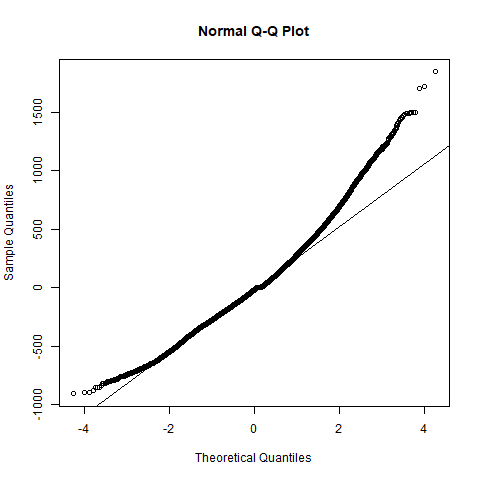
\includegraphics[width=\linewidth]{Images/anova_std.png}
 	\caption{Predichos contra los residuos}
 	\label{fig:anova_qq}
 \end{figure}
 
 En el gr\'afico de predichos contra los residuos (figura \ref{fig:anova_qq}), todos los puntos tienden 
 a estar sobre la una misma recta, aunque no est\'an  completamente alineados, y esto se pudiera deber al la
 sustitución de los datos faltantes o a la cantidad considerable de datos. La cantidad de puntos aberrantes
 es muy peque\~na con respecto al tama\~no de los datos por lo que podemos tolerar y seguir afirmando que se cumple el supuesto de normalidad.
 
 \begin{figure}[h!]
 	\centering
 	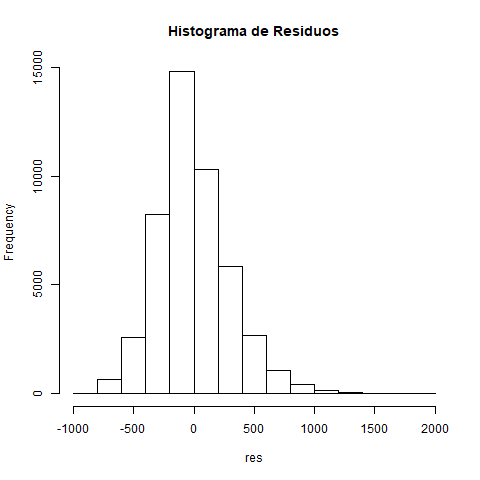
\includegraphics[width=\linewidth]{Images/anova_hist.png}
 	\caption{Histograma de residuos}
 	\label{fig:anova_hist}
 \end{figure}
 
 Finalmente, en la gr\'afica del histograma de residuos (figura \ref{fig:anova_hist}), dicha gr\'afica se asemeja decentemente a la normal con media $0$. Con lo cual afirmamos que se cumple el
 supuesto de normalidad.
 

 
 \subsubsection{Shapiro-Wilk, Bartlett y Durbin-Watson}
 
 El Test de Shapiro-Wilk no se pudo realizar por la gran cantidad de datos. Con lo cual, bas\'andonos
 en las pruebas gr\'aficas podemos asumir que el mismo se cumple y continuar con los dos test restantes.
 
 \begin{figure}[h!]
 	\centering
 	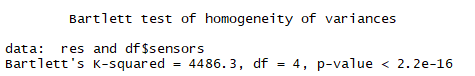
\includegraphics[width=\linewidth]{Images/anova_bartlett.png}
 	\caption{Test de igual varianza Bartlett}
 	\label{fig:anova_bartlett}
 \end{figure}
 
 Como muestra la prueba de la figura \ref{fig:anova_bartlett} (Test de Bartlett), el $p$-\textit{value} muestra que es significativa, con lo que rechazamos $H_0$, y no se cumple es supuesto de varianzas constantes. La prueba deja de tener validez.
 
 \begin{figure}[h!]
 	\centering
 	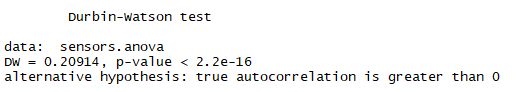
\includegraphics[width=\linewidth]{Images/anova_durbin.png}
 	\caption{Test Durbin-Watson}
 	\label{fig:anova_dwtest}
 \end{figure}
 
 Finalmente, y de igual forma la prueba de la figura \ref{fig:anova_dwtest} (Test Durbin-Watson) muestra que el test es significativo, por tanto no se cumple el supuesto de independencia.
 
 En conclusi\'on, los dos \'ultimos supuestos fallaron y por ende todos los resultados iniciales no son v\'alidos. A pesar del estado de los datos, se realiz\'o el an\'alisis. Concluimos que estos datos no son lo id\'oneos par una prueba de ANOVA.  
 
 \section{Conclusiones}
 
 Este equipo considera que la falta de valores presentes en la fuente impide que se pueda llegar a conclusiones específicas sobre los datos. Se recomienda realizar otra recopilación para un futuro estudio. Cualquier análisis con los datos actuales se considera como no confiable.
 
 Todos los códigos, resultados e imágenes presentes en este documento y relacionados con los experimentos se encuentran adjuntos dentro del directorio del proyecto.
 
\label{end}

\end{document}



%===================================================================================
